\newlength\bottomstripheight%
\setlength{\bottomstripheight}{.25\textheight}%
%
\begin{minipage}[t]{\textwidth}%
\vskip0pt%
\textcolor{BaseColor}{%
\rule{\textwidth}{.2mm}%
}\hfill%
%
%
\begin{minipage}[b][\bottomstripheight][b]{.48\textwidth}%
%
\cblock{BaseColor}{}{Training Results}{}%
\small%
We initialize a feed-forward architecture using a small percentage of its parameters. We train networks using standard SGD, sparsity enforcing ProxGD, and \LinBreg{}.
\begin{figure}
\begin{minipage}{.7\textwidth}%
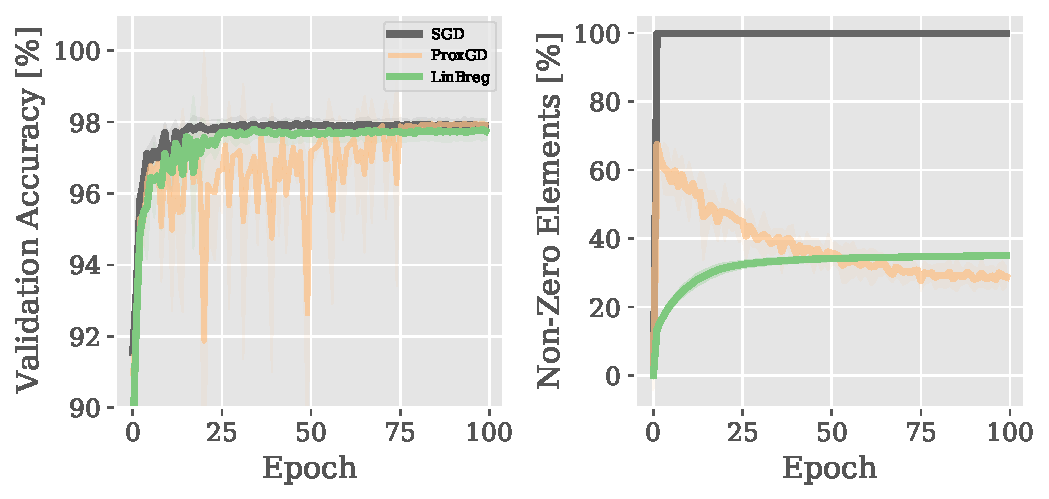
\includegraphics[width=\textwidth, trim= 0cm 0cm 0cm 0cm,clip]{atelier/SGDvsBreg_small.pdf}
\end{minipage}%
\begin{minipage}{.3\textwidth}%
\caption{\small Comparison of vanilla SGD, \LinBreg{}, and ProxGD.
The curves show mean validation accuracies and sparsity.}%
%
\vspace{100pt}

\end{minipage}%
\end{figure}%
%
%
%
\vfill%
Additionally, we compare ourselves to a variant of the LASSO \cite{tibshirani1996regression} regularizer on the CIFAR-10 dataset, employing a ResNet-18 network architecture.
% \cite{Krizhevsky09} 
%\cite{he2015delving}.
%
%
%
\begin{table}[htb]
\scriptsize
\begin{minipage}{.69\textwidth}%
\begin{tabularx}{\textwidth}{|c||c c|C C|}
Strategy & Optimizer & 
$\mathrm{N}_{\mathrm{total}}$ in [\%] & 
Test Acc&Train Acc\\
\hhline{|=====|}
\multirow{2}{*}{Vanilla}
&SGD with momentum &100.0&92.15&99.8\%\\
&Adam &100.0&93.6&100.0\%\\
\hhline{-----}
\multirow{2}{*}{Lasso}
        &Adam &99.7&91.1 &100\\
        &Adam + thresh.&3.0&90.0 &99.8\\
\hhline{-----}
\multirow{2}{*}{\textbf{\footnotesize Bregman}}
                &\LinBreg{} &5.5&90.9&99.5\\
                &\LinBreg{} + thresh.&3.4&90.2&99.4\\
\end{tabularx}
\end{minipage}%
\begin{minipage}{.01\textwidth}%
\phantom{2}
\end{minipage}%
%
\begin{minipage}{.3\textwidth}%
\caption{\small Sparsity levels and accuracies on the CIFAR-10 data set.}\label{tab:CIFAR}
\end{minipage}
\end{table}
%
%
%
%
%
%
\end{minipage}%
%
\hfill%
%
\tbox{%
\noindent\begin{minipage}[b][\bottomstripheight][b]{.005\textwidth}%
%
\begin{center}
\textcolor{BaseColor}{%
\rule{.2mm}{\bottomstripheight}%
}
\end{center}
\end{minipage}%
}%
%
\hfill%
%
%
%
%
%
%
%
\noindent\begin{minipage}[b][\bottomstripheight][b]{.48\textwidth}%
%
\cblock{BaseColor}{}{Neural Architecture Search with Bregman}{}%
\small%
% Initializing a sparse multi-layer perceptron and training this net in order to perform a denoising task reveals an autoencoder architecture \cite{bungert21}. 
Using group sparsity regularization $\func(\param) = \sum_{l=1}^L\norm{W^l}_{1,2}$ in a denoising task reveals an autoencoder architecture
\cite{bungert21}.

\begin{figure}%
\begin{minipage}{.3\textwidth}%
\caption{\small Architecture design for denoising: \LinBreg{} unveils an autoencoder.}
\vspace{210pt}

\end{minipage}%
\begin{minipage}{.7\textwidth}%
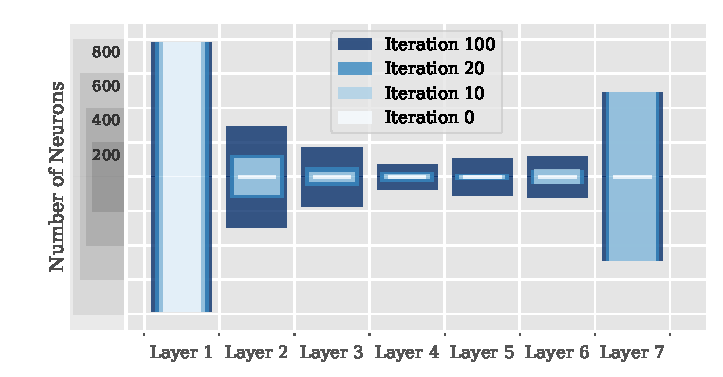
\includegraphics[trim = .7cm 0cm 0cm 0cm, clip, width=\textwidth]{atelier/Encoder.pdf}
\end{minipage}%
\end{figure}
%
%
%
\vfill%
\cblock{BaseColor}{BaseColorD}{\normalsize References}{%
\AtNextBibliography{\tiny}
\printbibliography[heading=none]
}
\end{minipage}%
\end{minipage}%
%
\begin{tikzpicture}[overlay]
\node[draw=BaseColor, fill=white, thick,minimum width=5cm,minimum height=5cm] (b) at (-38.5,-15.5){%

\includegraphics[width=4.5cm]{atelier/QR_Code.png}%
};
\end{tikzpicture}

